\documentclass[runningheads]{llncs}
%
\usepackage[T1]{fontenc}
% T1 fonts will be used to generate the final print and online PDFs,
% so please use T1 fonts in your manuscript whenever possible.
% Other font encondings may result in incorrect characters.
%
\usepackage{graphicx}
% Used for displaying a sample figure. If possible, figure files should
% be included in EPS format.
%
% If you use the hyperref package, please uncomment the following two lines
% to display URLs in blue roman font according to Springer's eBook style:
%\usepackage{color}
%\renewcommand\UrlFont{\color{blue}\rmfamily}
%
\begin{document}
%
\title{Reutilização de Software\thanks{Universidade de Évora.}}
%
%\titlerunning{Abbreviated paper title}
% If the paper title is too long for the running head, you can set
% an abbreviated paper title here
%
\author{Hugo Silva \email{m53080@alunos.uevora.pt}}

%
\authorrunning{H. Silva}
% First names are abbreviated in the running head.
% If there are more than two authors, 'et al.' is used.
%
\institute{Universidade de Évora, Évora, Portugal}
%
\maketitle              % typeset the header of the contribution
%
\begin{abstract}

O presente artigo aborda a reutilização de software como um pilar essencial no desenvolvimento de software. A reutilização de software consiste em reutilizar software existente para criar novos sistemas, permitindo assim, poupar tempo e recursos, aumentando a qualidade de software. É abordado os problemas associados à reutilização de software, como também as formas de minimizar os problemas que podem surgir devido à sua reutilização. O presente artigo aborda também o desenvolvimento de software baseado em componentes e em serviços, como as vantagens e benefícios associados à reutilização de software. Por fim, é realizada a conclusão sobre a reutilização de software.

\keywords{Reutilização de Software  \and Desenvolvimento baseado em componentes e serviços \and Problemas e soluções na reutilização de software.}
\end{abstract}
%
%
%
\section{Introdução}

\section{Reutilização de Software}

A reutilização de Software (Software Engineering (Ian Sommer Ville)) é uma estratégia utilizada em engenharia de software que tem como intuito reutilizar software existente.\par
A estratégia baseada em reutilização de Software têm sido adotada devido à necessidade de:


\begin{itemize}
    \item Menores custos de produção e manutenção de software;
    \item Maior velocidade de entrega dos sistemas informáticos;
    \item Aumento da qualidade do software.
\end{itemize}

As empresas cada vez mais veem o seu software como um ativo importante e têm vindo a  adotar a estratégia de reutilização do software, pois podem aumentar o seu retorno sobre os investimentos no software.\par
As unidades de software que podem ser reutilizadas podem ser de diferentes tamanhos, sendo:

\begin{itemize}
    \item Reutilização completa dos Sistemas;
    \item Reutilização da Aplicação;
    \item Reutilização de Componentes;
    \item Reutilização de Objectos e funções.
\end{itemize}

Todo o software e componentes que incluem funcionalidades genéricas podem ser potencialmente reutilizáveis, no entanto, existem certos softwares e componentes que por vezes são tão específicos que são muito custosos de modificar para a lógica de negócio pretendida.

\subsection{Vantagens e benefícios associados à reutilização de software}

Existem variadíssimas vantagens e benefícios associados à estratégia de reutilização de software, estes são:

\begin{itemize}
    \item Aceleração do desenvolvimento;
    \item Uso efectivo de especialistas;
    \item Maior confiança no software;
    \item Baixo custos de desenvolvimento;
    \item Redução da margem de erro na estimativa dos projectos;
    \item Conformidade com os padrões resulta em maior confiabilidade e menos erros.
\end{itemize}

\subsubsection{Aceleração do desenvolvimento.}

A reutilização de software pode acelerar o desenvolvimento do software, isto porque, o tempo de desenvolvimento e validação podem ser reduzidos. Trazer um sistema para o mercado o mais cedo possível é normalmente mais importante do que os custos totais de desenvolvimento.

\subsubsection{Uso efectivo de especialistas.}

A reutilização de software permite que os especialistas se foquem no desenvolvimento de novo software reutilizável que encapsula os seus conhecimentos, em vez de estarem constantemente a fazer o mesmo trabalho.

\subsubsection{Maior confiança no software.}

A reutilização de software estabelece uma maior confiança no software existente porque o software reutilizável normalmente já foi experimentado e testado anteriormente em sistemas reais, o que permitiu encontrar e corrigir erros de design e de implementação.

\subsubsection{Baixo custos de desenvolvimento.}

A reutilização de software pode permitir baixar os custos de desenvolvimento de software.. Isto porque, é possível reutilizar componentes e serviços já existentes, em vez de desenvolver software do zero. Reduzindo assim o tempo e recursos envolvidos no processo de desenvolvimento.  


\subsubsection{Redução da margem de erro na estimativa dos projectos.}

A reutilização de software ajuda na redução de margem de erro na estimativa dos projectos. Isto porque o software já passou por testes e validação em outros projetos, reduzindo assim o risco de erros ou problemas encontrados.\par
O custo do software existente já é conhecido, enquanto os custos de desenvolvimento estão sempre dependentes sobre o julgamento. Este é um importante factor a ter em consideração na gestão do projecto, porque reduz a margem de erro na estimativa.


\subsubsection{Conformidade com os padrões resulta em maior confiabilidade e menos erros.}

Alguns padrões, como padrões de interfaces, podem ser implementados como componentes reutilizáveis. Por exemplo, se um menu é implementado utilizando um componente reutilizável, todas as aplicações apresentam o mesmo formato de menu ao utilizador. O uso de padrões melhora a confiabilidade e usabilidade, pois, os utilizadores fazem menos erros quando apresentados com uma interface familiar.

\subsection{Problemas associados à reutilização de software}

A estratégia de reutilização de software, também têm certos problemas associados, estes são:

\begin{itemize}
    \item Criação, manutenção e uso de uma biblioteca de componentes;
    \item Encontrar, entender e adaptar componentes reutilizáveis;
    \item Aumento de custos de manutenção;
    \item Falta de suporte para ferramentas;
    \item Síndrome de “Não inventado aqui”.
\end{itemize}

\subsubsection{Criação, manutenção e uso de uma biblioteca de componentes.}

Popular um componente reutilizável de uma biblioteca e assegurar que os programadores possam utilizar a biblioteca pode ser bastante custoso. Os processos de desenvolvimento devem-se adaptar para garantir que a biblioteca é utilizada.

\subsubsection{Encontrar, entender e adaptar componentes reutilizáveis.}

Componentes de software têm de ser encontrados, entendidos e muitas das vezes adaptados para funcionarem num novo ambiente de desenvolvimento. Os engenheiros devem ser confiantes o suficiente para poderem encontrar um componente na biblioteca, antes de o incluírem no seu normal processo de desenvolvimento.

\subsubsection{Aumento de custos de manutenção.}

Se, por exemplo, o código fonte de um sistema ou componente reutilizável não estiver disponível, os custos de manutenção podem ser maiores. Isto porque, os elementos reutilizáveis do sistema podem-se tornar incompatíveis com as mudanças feitas ao sistema.

\subsubsection{Falta de suporte para ferramentas.}

Algumas ferramentas de software não suportam um desenvolvimento baseado em reutilização. Pode ser difícil ou impossível implementar estas ferramentas com um sistema de libraria de componentes. \par
No processo de desenvolvimento e design deste software, podem não ter considerado o desenvolvimento baseado em reutilização. É mais provável isto acontecer para ferramentas que suportam Embedded Systems do que sistemas Orientados a Objetos.

\subsubsection{Síndrome de “Não inventado aqui”.}

Alguns engenheiros de software preferem reescrever os componentes porque acreditam que os podem melhorar. Isto acontece parcialmente devido à falta de confiança e parcialmente devido ao facto que escrever software original é visto como algo mais desafiante que reutilizar o código de outros.

\subsection{Desenvolvimento de software baseado em componentes}


\subsection{Desenvolvimento de software baseado em serviços}



\subsection{Formas para minimizar os problemas que podem surgir devido à reutilização de software}

\section{Conclusão}


\section{First Section}
\subsection{A Subsection Sample}
Please note that the first paragraph of a section or subsection is
not indented. The first paragraph that follows a table, figure,
equation etc. does not need an indent, either.

Subsequent paragraphs, however, are indented.

\subsubsection{Sample Heading (Third Level)} Only two levels of
headings should be numbered. Lower level headings remain unnumbered;
they are formatted as run-in headings.

\paragraph{Sample Heading (Fourth Level)}
The contribution should contain no more than four levels of
headings. Table~\ref{tab1} gives a summary of all heading levels.

\begin{table}
\caption{Table captions should be placed above the
tables.}\label{tab1}
\begin{tabular}{|l|l|l|}
\hline
Heading level &  Example & Font size and style\\
\hline
Title (centered) &  {\Large\bfseries Lecture Notes} & 14 point, bold\\
1st-level heading &  {\large\bfseries 1 Introduction} & 12 point, bold\\
2nd-level heading & {\bfseries 2.1 Printing Area} & 10 point, bold\\
3rd-level heading & {\bfseries Run-in Heading in Bold.} Text follows & 10 point, bold\\
4th-level heading & {\itshape Lowest Level Heading.} Text follows & 10 point, italic\\
\hline
\end{tabular}
\end{table}


\noindent Displayed equations are centered and set on a separate
line.
\begin{equation}
x + y = z
\end{equation}
Please try to avoid rasterized images for line-art diagrams and
schemas. Whenever possible, use vector graphics instead (see
Fig.~\ref{fig1}).

\begin{figure}
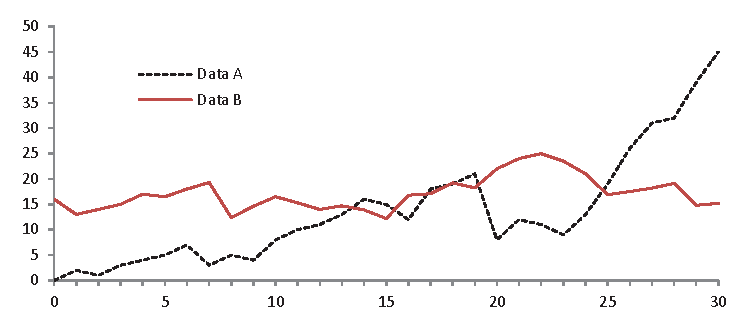
\includegraphics[width=\textwidth]{fig1.eps}
\caption{A figure caption is always placed below the illustration.
Please note that short captions are centered, while long ones are
justified by the macro package automatically.} \label{fig1}
\end{figure}

\begin{theorem}
This is a sample theorem. The run-in heading is set in bold, while
the following text appears in italics. Definitions, lemmas,
propositions, and corollaries are styled the same way.
\end{theorem}
%
% the environments 'definition', 'lemma', 'proposition', 'corollary',
% 'remark', and 'example' are defined in the LLNCS documentclass as well.
%
\begin{proof}
Proofs, examples, and remarks have the initial word in italics,
while the following text appears in normal font.
\end{proof}
For citations of references, we prefer the use of square brackets
and consecutive numbers. Citations using labels or the author/year
convention are also acceptable. The following bibliography provides
a sample reference list with entries for journal
articles~\cite{ref_article1}, an LNCS chapter~\cite{ref_lncs1}, a
book~\cite{ref_book1}, proceedings without editors~\cite{ref_proc1},
and a homepage~\cite{ref_url1}. Multiple citations are grouped
\cite{ref_article1,ref_lncs1,ref_book1},
\cite{ref_article1,ref_book1,ref_proc1,ref_url1}.

%
% ---- Bibliography ----
%
% BibTeX users should specify bibliography style 'splncs04'.
% References will then be sorted and formatted in the correct style.
%
% \bibliographystyle{splncs04}
% \bibliography{mybibliography}
%
\begin{thebibliography}{8}
\bibitem{ref_article1}
Author, F.: Article title. Journal \textbf{2}(5), 99--110 (2016)

\bibitem{ref_lncs1}
Author, F., Author, S.: Title of a proceedings paper. In: Editor,
F., Editor, S. (eds.) CONFERENCE 2016, LNCS, vol. 9999, pp. 1--13.
Springer, Heidelberg (2016). \doi{10.10007/1234567890}

\bibitem{ref_book1}
Author, F., Author, S., Author, T.: Book title. 2nd edn. Publisher,
Location (1999)

\bibitem{ref_proc1}
Author, A.-B.: Contribution title. In: 9th International Proceedings
on Proceedings, pp. 1--2. Publisher, Location (2010)

\bibitem{ref_url1}
LNCS Homepage, \url{http://www.springer.com/lncs}. Last accessed 4
Oct 2017
\end{thebibliography}
\end{document}
